\documentclass[twocolumn]{article}
\usepackage{fullpage}
\usepackage{amssymb}
\usepackage{amsmath}
\usepackage{enumerate}
\usepackage{graphicx}
\usepackage{url}
\usepackage[margin=2.2cm]{geometry}

\newcommand{\RR}{\mathbb{R}}
\newcommand{\ra}{\rightarrow}
\newcommand{\Wo}{W^{(1)}}
\newcommand{\Wt}{W^{(2)}}
\newcommand{\bo}{b^{(1)}}
\newcommand{\bt}{b^{(2)}}
\newcommand{\zr}{z^{(3)}}
\newcommand{\zt}{z^{(2)}}
\newcommand{\ar}{a^{(3)}}
\newcommand{\at}{a^{(2)}}
\newcommand{\ao}{a^{(1)}}
\newcommand{\dr}{\delta^{(3)}}
\newcommand{\dt}{\delta^{(2)}}
\newcommand{\xii}{x^{(i)}}
\newcommand{\pd}[2]{\ensuremath{\cfrac{\partial #1}{\partial #2}}}

\title{Properties of Autoencoders}
\author{%\sectionsize
    Justin Johnson \\
    \texttt{jcjohns@stanford.edu}
  \and
    Bharath Ramsundar \\
    \texttt{rbharath@stanford.edu}
}
\date{}

\begin{document}

\maketitle

\section{Introduction}
In recent years a variety of deep learning algorithms, including deep belief networks
\cite{hinton2006fast,lee2009convolutional} and deep neural networks, both convolutional
\cite{krizhevsky2012imagenet} and non-convolutional \cite{le2011building}. The types of
networks that are typically used in these applications are very complicated, and studying
their theoretical properties is very difficult.

Some approaches have utilized unsupervised
pretraining of deep neural networks in order to improve performance on classification tasks
\cite{le2011building}. One of the fundamental building blocks of this unsupervised pretraining
process is the sparse autoencoder. A single-layer autoencoder is a much simpler object than
an entire deep network, but even this relatively simple object has not been well-studied
theoretically.

In this project we aim to explore different varieties of autoencoders and to try and understand
why they work.

\vspace{-0.5pc}
\section{Sparse Autoencoder}
A sparse autoencoder is a neural network with a single hidden layer that attempts to learn the
identity function. The transfer function in these networks is nonlinear; in our experiments we use
the sigmoid transfer function $f(z)=1/(1+e^{-z})$.

Neural net weights are learned by minimizing an objective function consisting
of three terms. The first term is the $\ell^2$ reconstruction error of the training data.
The second term is $\ell^2$ regularization of the weight vectors. The third term constrains the
mean activation of each hidden layer neuron over the training set. The sparsity constraint can take
many forms, but our initial implementation uses a penalty of the form 
\[\sum_{j=1}^p\left(\rho\log\frac{\rho}{\hat\rho_j}+(1-\rho)\log\frac{1-\rho}{1-\hat\rho_j}\right)\]
where the hidden layer contains $p$ neurons, $\hat\rho_j$ is the mean activation of the $j$th hidden
layer neuron over the training set, and $\rho$ is a constant controlling the desired sparsity.
The weights of the trained network can be viewed as a feature transform for the training data.
We implemented this algorithm and ran it on the MNIST dataset \cite{lecun1998mnist}; the learned
feature transform is shown in Figure~\ref{fig:features}. Qualitatively, the learned features
roughly correspond to local object parts.

\vspace{-1.1pc}
\section{Equivalence with PCA}
An autoencoder that does not include the regularization or sparsity terms learns
a feature representation that is closely related to the principal components of
the training data \cite{bourlard1988auto}. We implemented this type of
autoencoder on the MNIST dataset and also ran principal component analysis on
the same dataset; the learned features can be seen in Figure~\ref{fig:features}.
The learned features appear to be qualitatively similar.

This equivalence between ``vanilla'' autoencoders and principal component
analysis suggests that the recent success of autoencoders is due to the
additional constraints placed upon their parameters. This motivates a more
in-depth analysis of the sparsity constraint.

\vspace{-1.1pc}
\section{Universal Approximation}
Neural networks with one hidden layer are capable of uniformly approximating
arbitrary continuous functions \cite{cybenko1989approximation}. This result,
which follows from a form of generalized fourier analysis, implies that neural
nets are capable of learning arbitrary classifiers. Note though, that
autoencoders are distinct from general neural networks, since autoencoders
attempt only to learn the identity. However, the universal approximation result
motivates the belief that autencoders can learn nontrivial, data-dependent forms
of the identity.

\vspace{-1pc}
\section{Sparse Linear Autoencoders}
We next considered a sparse linearized autoencoder where the transfer function
is simply the identity function. The objective function for this autoencoder is
the sum of the $\ell^2$ reconstruction error, an $\ell^2$ regularization term on
the network weights, and an $\ell^2$ sparsity constraint of the form
$\|\rho-\hat\rho\|_2^2$ where as above $\hat\rho_j$ is the mean activation of
the $j$th hidden unit on the training set. The learned features for this
autoencoder is shown in Figure~\ref{fig:features}.

\section{Discussion}
Our experimentation so far has led us to focus on the sparsity constraint of the
autoencoder.  For the remainder of the term we will consider other variants on
this constraint both on nonlinear and linearized networks. In particular, we
will experiment with $\ell^1$ and $\ell^2$ sparsity constraints on the nonlinear
network and an $\ell^1$ sparsity constraint on the linearized network. Depending
on the results of these experiments, we will attempt to understand the
theoretical implications of these sorts of constraints. In addition to the
linearized autoencoder, we would also like to experiment with networks whose
transfer function is a Taylor approximation to the sigmoid function.
  
\begin{figure*}
  \centering
  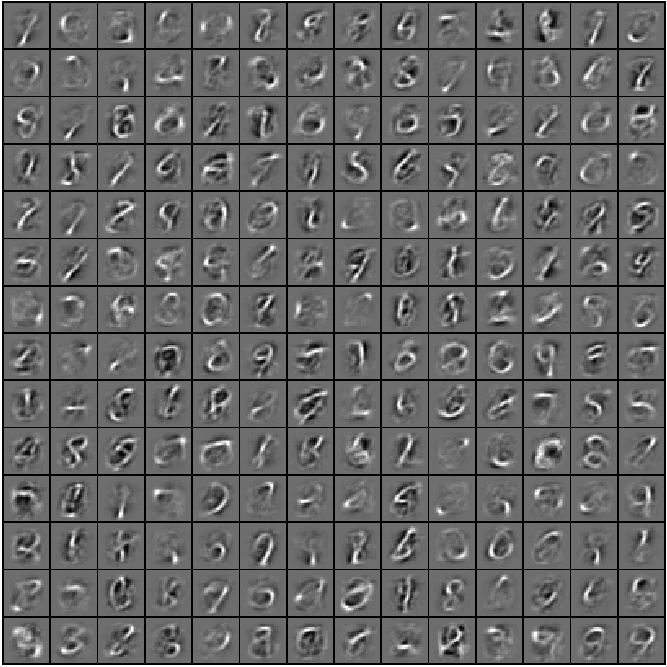
\includegraphics[width=0.45\textwidth]{sparsesigmoidnn.png}
  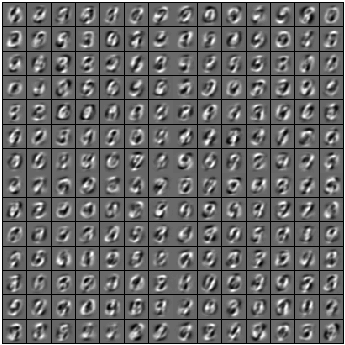
\includegraphics[width=0.45\textwidth]{linearnn.png}
  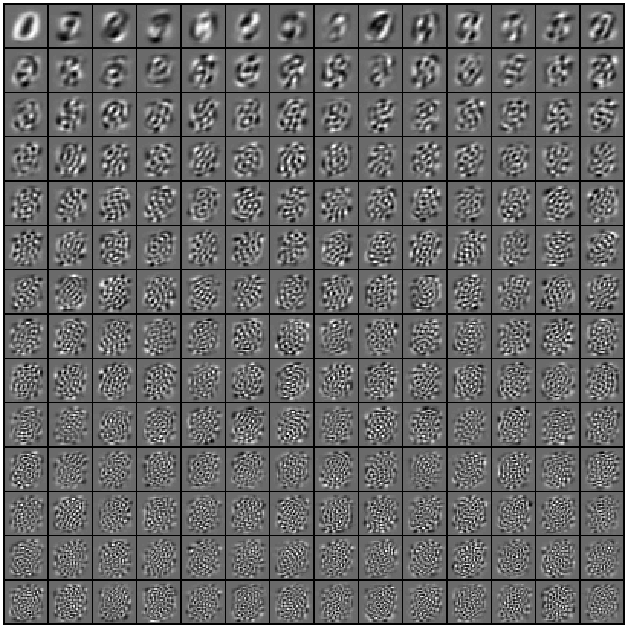
\includegraphics[width=0.45\textwidth]{pca.png}
  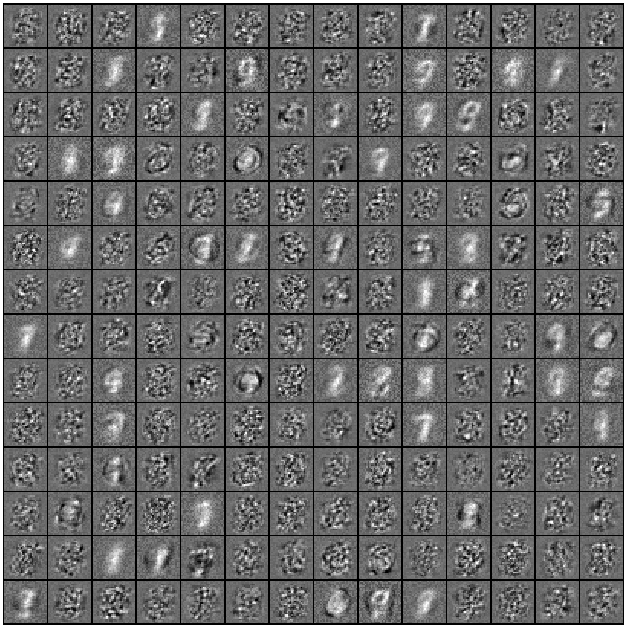
\includegraphics[width=0.45\textwidth]{nonlinearnn.png}
  \caption{Learned features for MNIST using different methods.
      Upper left: Sparse (nonlinear) autoencoder.
      Upper right: Sparse linear autoencoder.
      Lower left: Principal component analysis.
      Lower right: nonlinear autoencoder.
    }
  \label{fig:features}
\end{figure*}

\appendix
\section{Generalized Sparse Autoencoders}
In this section we describe a general framework for sparse autoencoders.
This is a generalization of the sparse autoencoder presented in \cite{ufldl-tutorial}.
An autoencoder is a neural network with a single hidden layer that attempts to learn the identity function
$\RR^n\ra\RR^n$. Let the hidden layer have $p$ units, and let $f:\RR\ra\RR$ be a differentiable activation
function. The neural network is parameterized by terms weights $\Wo\in\RR^{p\times n}$ and
$\Wt\in\RR^{n\times p}$ and bias terms $\bo\in\RR^p$ and $\bt\in\RR^n$. Given weight and bias terms, the
prediction on an input $x\in\RR^n$ is
\[h_{W,b}=f(\Wt f(\Wo x+\bo)+\bt)\]
Given training examples $x^{(1)},\ldots,x^{(m)}\in\RR^n$ the objective function for the generalized sparse
autoencoder is
\[J(W,b)=\frac1m\sum_{i=1}^m\ell(h_{W,b}(\xii),\xii)+\lambda\psi(W,b)+\beta\sum_{j=1}^p\phi(\hat\rho_j)\]
where we define
\[\hat\rho_j=\frac1m\sum_{j=1}^mf\left((\Wo_j)^T\xii+\bo_j\right)\]
to be the average activation of the $j$th hidden unit over the training set; here $(\Wo_j)^T$ is the
$j$th row of the matrix $\Wo$. In the sparse autoencoder objective function, $\ell:\RR^n\times\RR^n\ra\RR$
is a loss function that encourages the autoencoder to have low reconstruction error.
The function $\psi$ is a regularizer for the weight
and bias terms and the parameter $\lambda\in\RR$ controls the relative importance of the regularization.
Frequently we define $\psi(W,b)=\frac12\|\Wo\|^2_F+\frac12\|\Wt\|^2_F$ where $\|A\|_F$ is the Frobenius norm.
The function $\phi:\RR\ra\RR$ is the sparsity penalty, and the parameter $\beta\in\RR$ controls the relative
importance of the sparsity penalty.

We train a generalized sparse autoencoder using gradient descent.
For the remainder of the discussion we assume that $\ell(x,y)=\frac12\|x-y\|^2$;
this allows us to use the standard backpropogation algorithm to compute
the gradient of the reconstruction error term. For notational convenience, for $x\in\RR^n$ define
\begin{align*}
  \zt(x) &=\Wo x+\bo && \at(x) = f(\zt(x)) \\
  \zr(x) &=\Wt\at(x)+\bt && \ar(x) = f(\zr(x))
\end{align*}
In the standard backpropogation algorithm we define
\begin{align*}
  \dr(x) &= -(x-\ar(x))\odot f'(\zr(x)) \\
  \dt(x) &= \left((\Wt)^T\dr(x)\right)\odot f'(\zt(x))
\end{align*}
where $\odot$ is componentwise multiplication of vectors and $f'$ is applied componentwise.
Then the gradients of the reconstruction terms are given by
\begin{align*}
  \nabla_{W^{(k)}}\ell(h_{W,b}(x),x) &= \delta^{(k+1)}(x)a^{(k)}(x)^T \\
  \nabla_{b^{(k)}}\ell(h_{W,b)}(x),x) &= \delta^{(k+1)}(x)
\end{align*}
where $k\in\{1,2\}$ and we define $\ao(x)=x$.

Computing the gradient of $\psi(W,b)$ is typically straightforward; for example when
\[\psi(W,b)=\frac12\|\Wo\|_F^2+\frac12\|\Wt\|_F^2\] then $\nabla_{W^{(k)}}\psi(W,b)=W^{(k)}$ and
$\nabla_{b^{(k)}}\psi(W,b)=0$ for $k\in\{1,2\}$.

It remains to compute the gradient for the sparsity term.
Clearly $\nabla\phi(\hat\rho_j)=\phi'(\hat\rho_j)\nabla\hat\rho_j$ and $\nabla_{\bt}\hat\rho_j=0$ and
$\nabla_{\Wt}\hat\rho_j=0$ so we only need to compute $\nabla_{\bo}\hat\rho_j$ and $\nabla_{\Wo}\hat\rho_j$.
A bit of arithmetic shows that
\begin{align*}
  \pd{\hat\rho_j}{\bo_k} &= \begin{cases} 
      \frac1m\sum_{i=1}^mf'\left((\Wo_j)^T\xii+\bo_j\right) & j=k \\
      0 & \textrm{otherwise}
  \end{cases} \\
    \nabla_{\Wo_k}\hat\rho_j &= \begin{cases}
      \frac1m\sum_{i=1}^mf'\left((\Wo_j)^T\xii+\bo_j\right)\xii & j=k \\
      0 & \textrm{otherwise}
    \end{cases}
\end{align*}
A bit more arithmetic shows that if we modify the standard backpropogation algorithm and by setting
\[\dt_i(x) = \left(\sum_{j=1}^p\Wt_{ji}\dr_j(x)+\beta\phi'(\hat\rho_i)\right)f'\left(\zt_i(x)\right)\]
the the gradient of the sparse autoencoder objective function is simply
\begin{align*}
  \nabla_{b^{(k)}}J(W,b) &= \frac1m\sum_{i=1}^m\delta^{(k+1)}(\xii) + \lambda\nabla_{b^{(k)}}\psi(W,b) \\
  \nabla_{W^{(k)}}J(W,b) &= \frac1m\sum_{i=1}^m\delta^{(k+1)}(\xii)a^{(k)}(\xii)^T
    + \lambda\nabla_{W^{(k)}}\psi(W,b)
\end{align*}

\bibliographystyle{plain}
\bibliography{refs}


\end{document}
